\subsection{Princípio da demanda efetiva no médio prazo: um paradigma e duas alternativas?}
\label{Medium}

Até então, pode-se dizer que a teoria do crescimento liderado pela demanda enfrentava um impasse. Não conseguia conciliar estabilidade, distribuição funcional da renda exógena e grau de utilização da capacidade produtiva igual ao normal/planejado, aparentando uma trindade impossível do crescimento, conforme pode ser visto no diagrama \ref{diagrama}\footnote{Este diagrama é inspirado no ``trilema'' do crescimento apresentado por \textcite{cesaratto_neo-kaleckian_2015}.}.
Essa trindade impossível se mostrou falsa com o desenvolvimento do supermultiplicador sraffiano (SSM).

\begin{figure}[H]
	\caption{Trindade ``impossível''}
	\label{diagrama}
	\begin{center}
		\resizebox{0.45\textwidth}{!}{%
			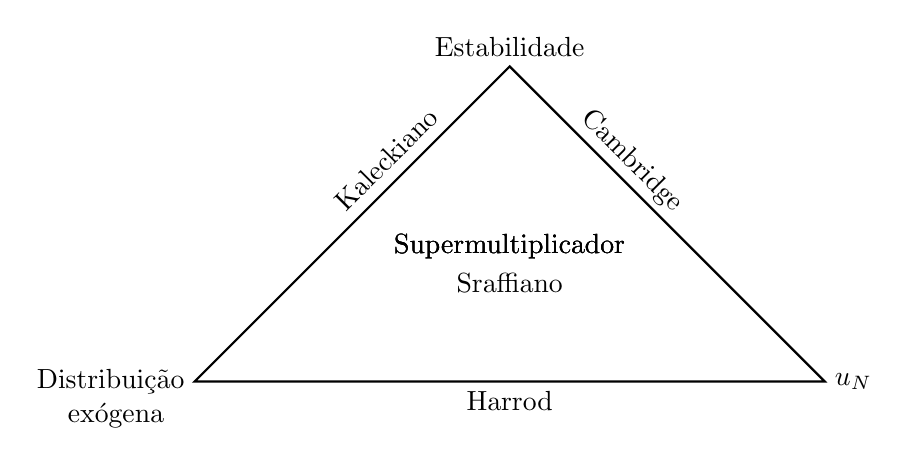
\begin{tikzpicture}[thick]
			\path[draw] (-4,0)  coordinate [label= left:Distribuição] (A)
			
			-- ( 0,4)  coordinate [label=above:Estabilidade] (C)
			-- ( 4,0)  coordinate [label=right:$u_N$] (B)
			-- cycle;
			\foreach \point in {A,B,C}
			\draw
			-- (0,2) node[anchor=north]{Supermultiplicador};
			\draw
			-- (-5,-0.15) node[anchor=north]{exógena};
			\draw
			-- (0,1.5) node[anchor=north]{Sraffiano};
			\draw
			-- (-1.75,3) node[anchor=north, rotate=45]{Kaleckiano};
			\draw
			-- (1.75,3) node[anchor=north, rotate=-45]{Cambridge};
			\draw
			-- (0,0) node[anchor=north]{Harrod};
			\end{tikzpicture}
		}
	\end{center}
	\caption*{\textbf{Fonte:} Elaboração própria}
\end{figure}
No entanto, da revisão da literatura verifica-se que tal mérito não se restringe ao SSM uma vez que uma vertente kaleckiana tem incluído gastos autônomos não criadores de capacidade produtiva por meio do princípio do ajuste do estoque de capital no \textbf{longo prazo}.
Sendo assim, é possível avançar em direção a um mapeamento de uma possível convergência entre os modelos sraffianos do tipo supermultiplicador e os modelos kaleckianos e então selecionar o caminho a ser seguido.
Antes de prosseguir, no entanto, cabe destacar que por serem modelos na fronteira da literatura, podem não ser representativos do que se entende por modelo kaleckiano e, por conta disso, serão denominados ``não-convencionais'' ao longo desta seção.

Em linhas gerais, tais modificações nos modelos kaleckianos estão associadas a algumas críticas envolvendo tanto a não convergência ao grau de utilização normal no longo prazo quanto a instabilidade decorrente da endogeinização do componente autônomo do investimento \cites{dallery_kaleckian_2007}{skott_theoretical_2012}{hein_harrodian_2012}.
A partir da contribuição de \textcite{allain_tackling_2015}, as alterações no modelo canônico têm a inclusão de gastos autônomos como denominador comum.
Uma vez introduzidos estes gastos, a poupança agregada torna-se
$$
\frac{S}{Y} = s - \frac{Z}{Y}
$$
Neste ponto, \textcite[p.~10]{allain_tackling_2015} segue \textcite{serrano_sraffian_1995} em que a presença dos gastos autônomos possibilitam o ajuste da identidade entre investimento e poupança pela participação desses gastos na renda e não por mudanças no grau de utilização. 

Dito isso, o autor prossegue para o médio prazo\footnote{
	Uma das distinções \textcite{allain_tackling_2015} são as caracterizações do curto, médio e longo prazo. O primeiro é definido pela não alteração dos gastos autônomos enquanto o segundo pode ser definido como aquele que tais gastos crescem a taxa exogenamente determinada. Por fim, o longo prazo é caracterizado por uma função de investimento Harrodiana com o grau de utilização convergindo ao desejado. Vale pontuar a distinção com a temporalidade encontrada em \textcite{freitas_growth_2015} em que a convergência ao grau de utilização normal se dá na \textit{fully-adjusted position} enquanto a convergência da taxa de crescimento a $g_Z$ é dada no longo prazo. Para manter a comparatividade entre os modelos kalekicanos não-convencionais, adota-se a caracterização de \textcite{allain_tackling_2015} ao longo desta seção.
} em que a participação dos gastos autônomos na renda ($z$)\footnote{A rigor, o autor define essa participação dos gastos autônomos normalizados pelo estoque de capital e não pela renda, mas tal apresentação não altera a exposição ao longo do texto.} varia de acordo com a diferença entre as taxas de crescimento dos gastos autônomos e a efetiva ($g$):
\begin{equation}
\Delta z = (g_Z - g)\cdot z_{t-1}
\end{equation}
Assim, quando a taxa de crescimento efetiva da economia se difere da taxa de crescimento dos gastos autônomos ($g\neq g_Z$)  haverá uma variação na participação dos gastos autônomos ($\Delta z$), impactando a demanda agregada e a poupança. No médio prazo, em que a taxa de crescimento converge a taxa dos gastos autônomos, o mecanismo de ajuste é encerrado e o grau de utilização é dado por:

\begin{equation}
u = \frac{g_z - \gamma}{\gamma_u} + u_N
\end{equation}
Esta equação evidencia que se, e somente se, a expectativa tendencial de crescimento ($\gamma$) for igual à taxa de crescimento dos gastos autônomos, o grau de utilização convergirá ao normal no médio prazo e, portanto, é meramente acidental. No entanto, a convergência do grau de utilização ao normal é uma característica do longo prazo que decorre do princípio de ajuste do estoque de capital em que a taxa de crescimento esperada se adequa aos distanciamentos entre o grau de utilização efetivo e normal. No entanto, para evitar o deflagrar da instabilidade no modelo kaleckiano canônico é necessário que o investimento deixe de ser autônomo: 
\begin{equation}
\label{eqAllain}
\Delta \gamma = \phi\gamma_u(u - u_N)
\end{equation}
em que $\phi$ é um fator de ajuste positivo e suficientemente pequeno\footnote{
	Além disso, \textcite[p.~14]{allain_tackling_2015} argumenta que a novidade  é o parâmetro  de ajustamento positivo ($\phi > 0$) que além de não implicar na instabilidade Harrodiana, é também condição de estabilidade do modelo.
}.
Dito isso e partindo do equilíbrio de médio prazo e supondo um aumento na taxa esperada de crescimento, obtém-se um cenário em que a taxa efetiva de crescimento é maior que a taxa de crescimento dos gastos autônomos. Como consequência, a participação dos gastos autônomos na renda diminui de modo que  a poupança agregada aumenta. Essa redução, por sua vez, tem um efeito negativo tanto sobre a taxa de crescimento efetiva quanto sobre o grau de utilização. Esse processo se esgota com a taxa de crescimento efetiva se ajustando a taxa de crescimento dos gastos autônomos ($g = g_z$) mas com um grau de utilização menor  (equilíbrio de médio prazo reestabelecido). 

No longo prazo, instaura-se o princípio do ajuste do estoque de capital de modo que o grau de utilização converge ao normal ($u \to u_N$) em que: (i) Mudanças na distribuição de renda geram alterações no nível, mas não na taxa de crescimento, eliminado o paradoxo dos custos; (ii) o mesmo vale para alterações na propensão marginal a poupar e o paradoxo da parcimônia; (iii) o grau de utilização converge ao normal no longo prazo e não é afetado por modificações no comportamento do investimento/poupança dada a introdução dos gastos autônomos que crescem exogenamente e dado o ajuste na propensão marginal a investir e (iv) aumento da taxa de crescimento dos gastos autônomos tem impactos positivos sobre a taxa de acumulação\footnote{
	A convergência do grau de utilização ao nível normal implica na eliminação dos paradoxos kaleckianos em termos de taxas. Além disso, vale destacar que tal convergência decorre de uma das soluções do modelo é a equivalência entre o componente autônomo do investimento e a taxa de crescimento dos gastos autônomos. Como consequência indireta da crítica do supermultiplicador sraffiano, não raro encontram-se modelos kaleckianos (não-convencionais) com convergência ao grau de utilização normal que destacam a manutenção dos resultados canônicos na média:
	
	\begin{citacao}
		Thus, \textbf{on average}, the rate of utilization and the growth rate of the
		economy are higher than at the starting and terminal points of the traverse. Thus, what
		these Sraffians are telling us is that more attention should be paid to the average values
		achieved during the traverse than to the terminal points.
		\cite[p.~408, grifos adicionados]{lavoie_post-keynesian_2015}
	\end{citacao}
	
}. Em linha com \textcite{fagundes_role_2017}, argumenta-se que no \textbf{longo prazo} os modelos kaleckianos não-convencionais respondem suficientemente bem à convergência do grau de utilização sem incorrer na instabilidade, ou seja,
$$
\gamma = g = g_Z \Leftrightarrow u \to u_N
$$
%%%%%%%%%%%%%%%%%%%%%%%%%%%%%%% Início Fagundes e Freitas %%%%%%%%%%%%
Para encerrar essa discussão, é feita uma comparação entre as duas alternativas restantes, qual sejam, kalekiana não-convencional e sraffiana.  Diante disso, existem duas questões importantes em aberto: (i) dadas as hipóteses compartilhadas, qual a distinção fundamental entre ambos os modelos? (ii) dados os objetivos desta investigação, qual modelo a ser adotado? 

O primeiro ponto pode ser respondido de forma mais direta: a principal diferença é a autonomia do investimento no curto e médio prazo.  Resumidamente, se o investimento produtivo for induzido, a convergência ao grau de utilização normal é uma derivação do princípio do ajuste do estoque de capital e, dados certos limites, a capacidade produtiva se ajusta à demanda efetiva:

\begin{citacao}
	\textit{Indeed, the true reason for the lack of balance between capacity and demand in the Oxford theory [Modelos kaleckianos] in the long run is actually much simpler. As we have seen above in this theory, in the long run the level of output adapts itself to the level of aggregate demand. The level of productive capacity, however, cannot adjust to this level of aggregate demand because current capacity has already been determined as the result of previous autonomous investment. Hence it is the idea that investment is \textbf{autonomous} and not \textbf{anything related to oligopoly} or competition that explain the long-run discrepancies between capacity and demand.}
	\cite[p.~120, grifos adicionados]{serrano_sraffian_1995}
\end{citacao}
Por outro lado, se o investimento possuir um componente autônomo, como nos modelos kaleckianos convencionais, a demanda efetiva se ajusta à capacidade produtiva que está definida aprioristicamente:
\begin{citacao}
	\textit{Note that from our definition of capacity generating investment expenditures, it follows that when this type of investment is induced, productive capacity is necessarily a consequence of the evolution of effective demand. On the other hand, when capacity generating investment is autonomous it is productive capacity that emerges as a necessary consequence of (autonomous) investment. […] Indeed, the view that capacity of each sector is adjusted to normal level of effectual demand in every long-period position, necessary implies treating the long-period level of capacity generating investment as an endogenous magnitude.} \cite[p.~77]{serrano_sraffian_1995}
\end{citacao}
Como mostrado ao longo desta seção, isso deixa de ser o caso nos modelos kaleckianos com investimento induzido no longo prazo.

Para responder a segunda questão, resta esclarecer um possível ponto de estranhamento. O principal objetivo desta pesquisa é investigar os determinantes do ciclo econômico norte americano e desenvolver um modelo que replique alguns dos fatos estilizados. Sendo este o caso, a ênfase na discussão de modelos de longo prazo parece ser desconexa. 
No entanto, como mencionado na introdução, os modelos elegíveis são aqueles reportam alguns fatos estilizados (\textit{e.g.} relação positiva entre taxa de investimento e crescimento)  no curto, médio e longo prazo.
Desse modo, optar por modelos que se mostram adequados para o curto e longo prazo, mas não para o médio-prazo se mostra questionável uma vez que a validade dos resultados está restrita a uma certa temporalidade. 

%TODO Rever temporalidade
Os modelos restantes representam alguns fatos estilizados no curto prazo e na posição planamente ajustada (equivalente ao ``longuíssimo'' prazo kaleckiano). Resta verificar se o mesmo vale enquanto a propensão marginal a poupar não está ajustada (denominado aqui por  \textbf{médio prazo})\footnote{Esta parte da exposição é inspirada na contribuição de \textcite{fagundes_role_2017} no que diz respeito ao médio prazo.}. 
%TODO Rever se o tratamento de médio prazo está adequado
%Dito isso, dentre os modelos kaleckianos com gasto autônomo e principio de ajuste do estoque de capital e supermultiplicador sraffiano, resta selecionar aquele reproduza o fato estilizado da relação positiva entre taxa de investimento e taxa de crescimento. 
Dito isso, seja $i$ a taxa de investimento, $\gamma_A$ a parcela autônoma e $h$ a parcela induzida do investimento (das firmas) de modo que a representar a função de acumulação kaleckiana pode ser reescrita como\footnote{
	As etapas são:
	$$
	\frac{I}{K}  = \gamma + \gamma_uu - \gamma_uu_N
	$$
	
	$$
	\gamma_A = \gamma - \gamma_uu_N
	$$
	
	$$
	I = (\gamma_A + \gamma_uu)K
	$$
	
	$$
	\gamma_u\cdot u \cdot K \equiv \gamma_u\frac{Y}{Y_{FC}}K \equiv \gamma_u\cdot v\cdot Y
	$$
	
	$$
	I = \gamma_A\cdot K + \gamma_u\cdot v\cdot Y
	$$
}

\begin{equation}
\tag{kaleckiana}
I = \gamma_A\cdot K + h\cdot Y
\end{equation}
enquanto a do supermultiplicador (adiante, SSM) continua sendo

\begin{equation}
\tag{SSM}
I = h\cdot Y
\end{equation}
Como destacado na seção \ref{SecHarrod}, na ausência de gastos autônomos, a propensão marginal e média a poupar são iguais e, portanto, no modelo kaleckiano convencional, a taxa de investimento é determinada pela taxa de poupança definida exogenamente. Incluindo os gastos autônomos neste modelo, obtém-se:

$$
i = \frac{i_{Trad}\gamma_A + hz}{\gamma_A + z}
$$
em que $i_{Trad}$ denota, tal como em \textcite{fagundes_role_2017}, a taxa de investimento no modelo kaleckiano canônico. Nos modelos kaleckianos não-convencionais, a ausência dos gastos autônomos implica na volta ao modelo kaleckiano convencional enquanto no supermultiplicador retorna-se ao \textcite{harrod_essay_1939}. Mais uma vez, a introdução de tais gastos não é capaz, por si só, de eliminar a instabilidade, mas sim pela modificação da função investimento \textit{à la} acelerador flexível cuja alteração é feita somente no longo prazo nos modelos derivados de \textcite{allain_tackling_2015}. 

Prosseguindo com a exposição e analisando o equilíbrio de \textit{steady growth} com gastos autônomos ($Z > 0$), verifica-se que no médio prazo dos modelos kaleckianos não-convencionais ($g\to g_Z$), a taxa de investimento ($i_{MR}$) é dada por:
\begin{equation}
\label{investoFagundes}
i_{MR} = \frac{h\cdot g_Z}{g_Z - \gamma_A}
\end{equation}
Diante deste resultado, \textcite{fagundes_role_2017} argumentam que a inclusão dos gastos autônomos no modelo não garante a convergência do grau de utilização ao normal. Para que tal tendência ocorra, por sua vez, é necessário que a participação da parcela autônoma do investimento convirja a zero ($\gamma_A \to 0$) e isto ocorre no modelo de \textcite{allain_tackling_2015}. 
No entanto, \textcite{fagundes_role_2017} reportam que de acordo com este modelo, uma economia que cresce a taxas maiores é aquela que apresenta uma menor taxa de investimento que, por sua vez, contraria os fatos estilizados. Supondo, por simplificação, que as variações são infinitesimais, isto pode ser explicitado em termos da equação \ref{investoFagundes} por derivadas parciais:
$$
\frac{\partial i_{MR}}{\partial g_Z} = - \frac{\gamma_A h}{[g_Z - \gamma_A]^2} < 0 \Leftrightarrow \gamma_A > 0
$$
Além disso, os autores pontuam um problema de ``dupla indentidade'' nos modelos \textit{à la} \textcite{allain_tackling_2015} decorrente das diferentes condições de equilíbrio, um com e outro sem gastos autônomos, cujos padrões de crescimento são mutualmente excludentes. No primeiro, obtém-se um regime liderado pelo investimento produtivo, mas incapaz de gerar a tendência do grau de utilização ao normal e de destacar a importância dos gastos autônomos ($Z\to 0$). No outro, ocorre o inverso, um regime liderado pelos gastos autônomos ($\gamma_A \to 0$), mas que evidencia uma relação negativa entre crescimento e taxa de investimento. Ambos os casos contrariam alguns fatos estilizados. Portanto, a aceitação a conclusão de \textcite[p.~13]{fagundes_role_2017} é imediata:

\begin{citacao}
	
	[I]f we think of such a model as an intermediate step towards the long-run model, then we
	believe that there is no problem in using it. The problem occurs when we think of the medium-run
	model as a contribution to the understanding of economic reality in itself, independent from the long-run model.
\end{citacao}
Neste ponto, o trecho a seguir é esclarecedor:

\begin{citacao}
	What the supermultiplier adds to the neo-Kaleckian framework is a plausible mechanism for explaining phases
	of the business cycle when the output share of capacity investment is rising amidst robust rates of output growth. \cite[p.~9]{fiebiger_trend_2017}
\end{citacao}

Resta checar se a alternativa pelo SSM incorre nos mesmos problemas. Para isso, basta verificar os resultados para o caso em que o investimento é completamente induzido. Como a alternativa kaleckiana com gastos autônomos pode ser considerada como híbrida entre o modelo kaleckiano convencional e o SSM, basta substituir $\gamma_A = 0$ na equação \ref{investoFagundes}, obtendo:
$$
i_{MR} = \frac{I}{Y} =  h
$$
Seguindo a proposta do supermultiplicador em que o investimento é completamente induzido:
$$
g = \frac{h\cdot u}{v} \Rightarrow h^* = i_{MR} = \frac{g_Z\cdot v}{u}
$$

$$
\frac{\partial i_{MR}}{\partial g_Z} = \frac{v}{u} > 0
$$
Portanto, a relação negativa entre crescimento e taxa de investimento deixa de existir e isso não é feito às custas da não convergência do grau de utilização ou da relevância dos gastos autônomos no longo prazo. 
Diante desta discussão, conclui-se que o modelo do SSM não é incompatível para analisar o médio prazo ou restrito ao longo prazo como afirma \textcite{nikiforos_comments_2018}. Com isso, elege-se o supermultiplicador sraffiano como o mais adequado para atender os objetivos desta pesquisa. 


%TODO TRANSIÇÃO SEÇÃO SEGUINTE



